
\documentclass[12pt,letterpaper,notitlepage]{article}
\usepackage{graphicx}
\usepackage{float}
\usepackage{epsfig,epsf}
\usepackage{epstopdf}
\usepackage{curves}
\usepackage{hyperref}
% The following packages are important as they allow to write certain mathematical expressions.
\usepackage{amsmath}
\usepackage{amssymb}
\usepackage{color}
% To write a code in a LaTeX document you need:
\usepackage{listings}
\definecolor{dkgreen}{rgb}{0,0.6,0}
\definecolor{dkblue}{rgb}{0,0.0,0.6}
\definecolor{dkred}{rgb}{0.9,0.0,0.1}
%% Own definitions:
\newcommand{\BEq}{\begin{eqnarray}}
\newcommand{\EEq}{\end{eqnarray}}
\newcommand{\BEqn}{\begin{eqnarray*}}
\newcommand{\EEqn}{\end{eqnarray*}}
\newcommand{\BM}{\begin{subequations}}
\newcommand{\EM}{\end{subequations}}
\newcommand{\BEqM}{\begin{subequations}\begin{eqnarray}}
\newcommand{\EEqM}{\end{eqnarray}\end{subequations}}
\newcommand{\Bitem}{\begin{itemize}}
\newcommand{\Eitem}{\end{itemize}}
\newcommand{\Ben}{\begin{enumerate}}
\newcommand{\Een}{\end{enumerate}}
%% Greek letters:
\renewcommand{\a}{\alpha}
\renewcommand{\b}{\beta}
\newcommand{\D}{\Delta}
%% Colors:
\newcommand{\TB}[1]{\textcolor{blue}{#1}}
\newcommand{\TR}[1]{\textcolor{red}{#1}}
\newcommand{\bm}[1]{\mbox{\boldmath $#1$}}
\newcommand{\non}{\nonumber\\}
%% Some simplified expressions:
\def\eps{\varepsilon}
\def\r{\right}
\def\l{\left}
\def\p{\partial}
\def\d{\delta}
\newcommand{\ta}{\mbox{$\theta$}}
\newcommand{\ve}{\mbox{${\cal E}$}}
\newcommand{\etab}{\bar{\eta}}
\newcommand{\sg}{\tilde{\sigma}}
\newcommand{\tap}{\mbox{$\theta'$}}
\newcommand{\tta}{\mbox{$\tilde{\theta}$}}
\newcommand{\ttap}{\mbox{$\tilde{\theta}'$}}
\newcommand{\taz}{\mbox{$\theta_0$}}
\newcommand{\phip}{\mbox{$\phi'$}}
\newcommand{\tphi}{\mbox{$\tilde{\phi}$}}
\newcommand{\tphip}{\mbox{$\tilde{\phi}'$}}
\newcommand{\ty}{\mbox{$\tilde{y}$}}
\newcommand{\gb}{\mbox{$\bar{\gamma}$}}
\newcommand{\gone}{\mbox{$\gamma_1$}}
\newcommand{\gtwo}{\mbox{$\gamma_2$}}
\newcommand{\phiz}{\mbox{$\phi_0$}}
\newcommand{\Nf}{\mbox{$N_f$}}
\newcommand{\Nv}{\mbox{$N_v$}}
\newcommand{\qt}{\mbox{$\tilde{q}$}}
\newcommand{\qa}{\mbox{$q_\alpha$}}
\newcommand{\tqa}{\mbox{$\tilde{q}_\alpha$}}
\newcommand{\dqa}{\mbox{$\delta q_\alpha$}}
\newcommand{\pqa}{\mbox{$\partial_{u} q_\alpha$}}
\newcommand{\pqta}{\mbox{$\partial_{u} \tilde{q}_\alpha$}}
\newcommand{\pdqa}{\mbox{$\partial_{u}\delta q_\alpha$}}
\newcommand{\sn}{\mbox{${\rm sn}$}}
\newcommand{\cn}{\mbox{${\rm cn}$}}
\newcommand{\dn}{\mbox{${\rm dn}$}}
\newcommand{\cd}{\mbox{${\rm cd}$}}
%%% Creation, destruction operators:
\newcommand{\cks}{\mbox{$c_{{\bf k},\sigma}$}}
\newcommand{\cksd}{\mbox{$c_{{\bf k},\sigma}^\dagger$}}
\newcommand{\cku}{\mbox{$c_{{\bf k},\uparrow}$}}
\newcommand{\ckd}{\mbox{$c_{-{\bf k},\downarrow}$}}
\newcommand{\ckud}{\mbox{$c_{{\bf k},\uparrow}^\dagger$}}
\newcommand{\ckdd}{\mbox{$c_{-{\bf k},\downarrow}^\dagger$}}

\begin{document}

\lstset{language=Fortran,tabsize=4,numbers=left,numberstyle=\tiny,basicstyle=\ttfamily\small\color{dkblue},stringstyle=\ttfamily\color{blue},keywordstyle=\rmfamily\color{dkred}\bfseries\emph,backgroundcolor=\color{white},commentstyle=\color{dkgreen}}


\title{%
	Midterm 1, Problem 2  \\
\large Computational Physics - Phys 562}
\author{Benjamin Deutsch  \\
Department of Physics\\
California State University Long Beach}
\date{\today }

  
\maketitle



\begin{abstract}     
\end{abstract}

\section{Introduction}

In physics the use of differential equations is inescapable, this is even more true for the more instinctive, coupled set of motion equations. So it would follow that a way of attacking these computationally would be of great importance. There exists many ways to do this, even some still being a large body of current research, however the Runge-Kutta Method (RK4) has been used repeatedly and has gained fame in the its simplicity. A small problem arises in this computation, when global errors are large, run time is low, meaning that the error for each step accumulate over time. To avoid this inconsistency we make use of the adaptive Runge-Kutta method or RK45, this method uses a adaptive step size whos effects are two fold, one in truncation of the local error it stops a permeation of errors throughout each iteration. Second in correcting this error it optimizes the step size for the smallest error. This creates a shorter runtime and more useful output data. 
\\
\\
In the second problem of the computational midterm we are ask to explore this method by way of a sun moon earth system. Given the equations of motions, needed by the RK45 method, we can interpolate and approximate the motion of the celestial bodies for a given unit of time, here we will investigate the effects of one year. To demonstrate the three body problem, we use the fortran programming environment whose power of numerically irritative output will be then plotted to show to motions of the planet system.     

\section{The Math and Theory}

For the assignment we are asked to use the three bodied   seen here,
\\
	\begin{align}
\ddot{x}_1 &= -G m_2 \frac{x_1 - x_2}{|x_1 - x_2|^3} - G m_3 \frac{x_1 - x_3}{|x_1 - x_3|^3} \\
\ddot{x}_2 &= -G m_3 \frac{x_2 - x_3}{|x_2 - x_3|^3} - G m_1 \frac{x_2 - x_1}{|x_2 - x_1|^3} \\
\ddot{x}_3 &= -G m_1 \frac{x_3 - x_1}{|x_3 - x_1|^3} - G m_2 \frac{x_3 - x_2}{|x_3 - x_2|^3}
	\end{align}
\\
This is true with the movement of three different bodies, however since in our calculations the sun is left at the zero point with no movement. We need only two in vector form;
	\begin{align}
		\cfrac{d^2\vec{r_1}}{dt^2} &= -G m_2 \frac{\vec{x_1} - \vec{x_2}}{|\vec{x_1} - \vec{x_2}|^3} - G m_3 \frac{\vec{x_1}}{|\vec{x_1}|^3} \\
		\cfrac{d^2\vec{r_2}}{dt^2} &= -G m_2 \frac{\vec{x_2}}{|\vec{x_2}|^3} - G m_3 \frac{\vec{x_2} - \vec{x_1}}{|\vec{x_2} - \vec{x_1}|^3}
  	\end{align}
\\
Here we have a set of differentials to describe the sun earth moon system for use in the RK45 method.  

\section{The code}
Here, two different files were used, one which houses the main routine and another that contains the {\tt subroutine} for the RK45 method label {\tt rk45step.f95}. The main routine was setup in a standard way, with the addition of a module header so that the variables and parameters specified there could be shared to the subroutine. An important array to be defined is the \textbf{y} array which will house all changing values for the initial conditions below to be transferred between the subroutine. Independent values for position and velocity (\textbf{x,y,z}) given by literature were then placed into the corresponding array location for the earth and moon. A do loop was implemented next to write these values to an outer file and here with use of the RK45 subroutine the process would step forward.
To understand the motions of the now simplified three body problem, we must orient each body relative to each other, a simple way to do this assigning vectors for each of the radii (with the sun left out as explained above). The two bodies motion around the sun is a straight forward entry into the final equations above with the ex dot product arrays replacing the difference in positions, even though the moon's contribution is negligible it has been enter here nonetheless. This is done primary for inspection of other bodied systems, whos effects may not be so minimal in affecting the motion.      
\section{Results and Conclusion}	
	\begin{figure}[H]
		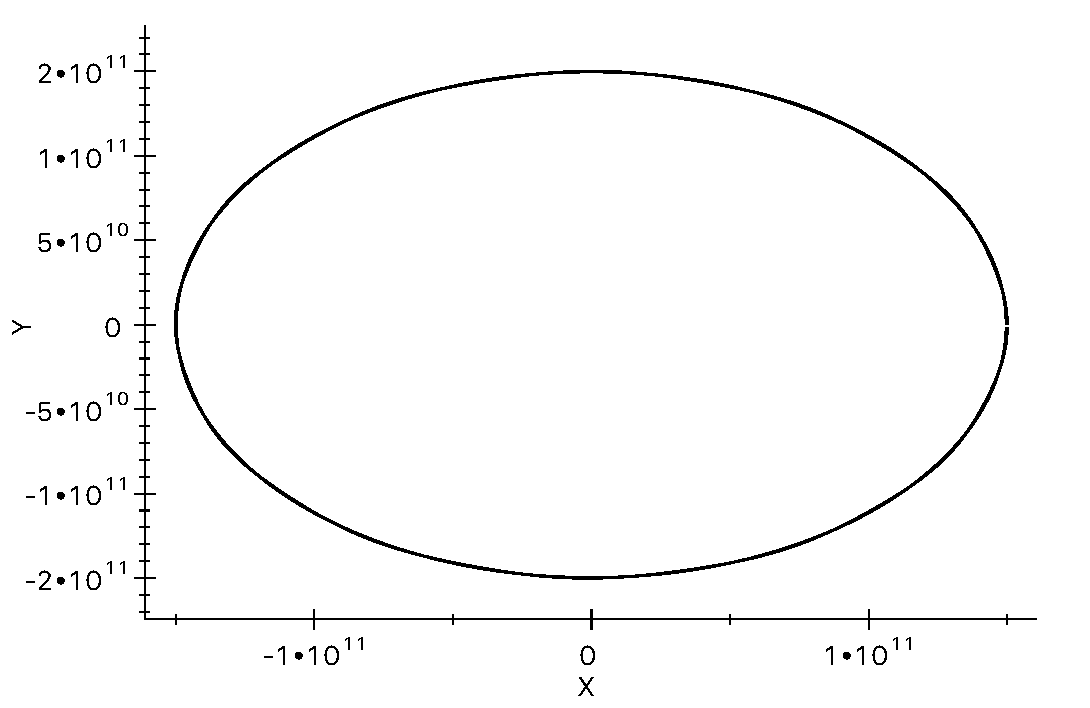
\includegraphics[width=1.\textwidth]{looper.pdf}
		\caption{The motion of the three bodied system, with the Sun in the center}
	\end{figure}  
	\begin{figure}[H]
		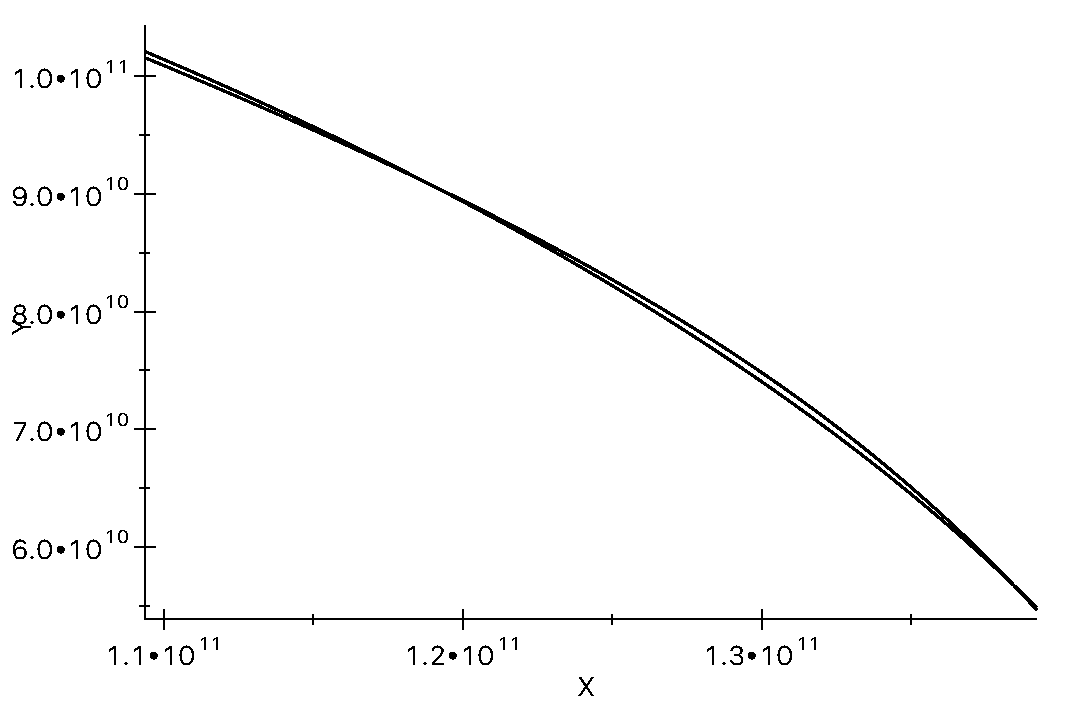
\includegraphics[width=1.\textwidth]{zoomlooper.pdf}
		\caption{Detailed look at the Moon motion about the Earth} 
	\end{figure}  
	\begin{figure}[H]
		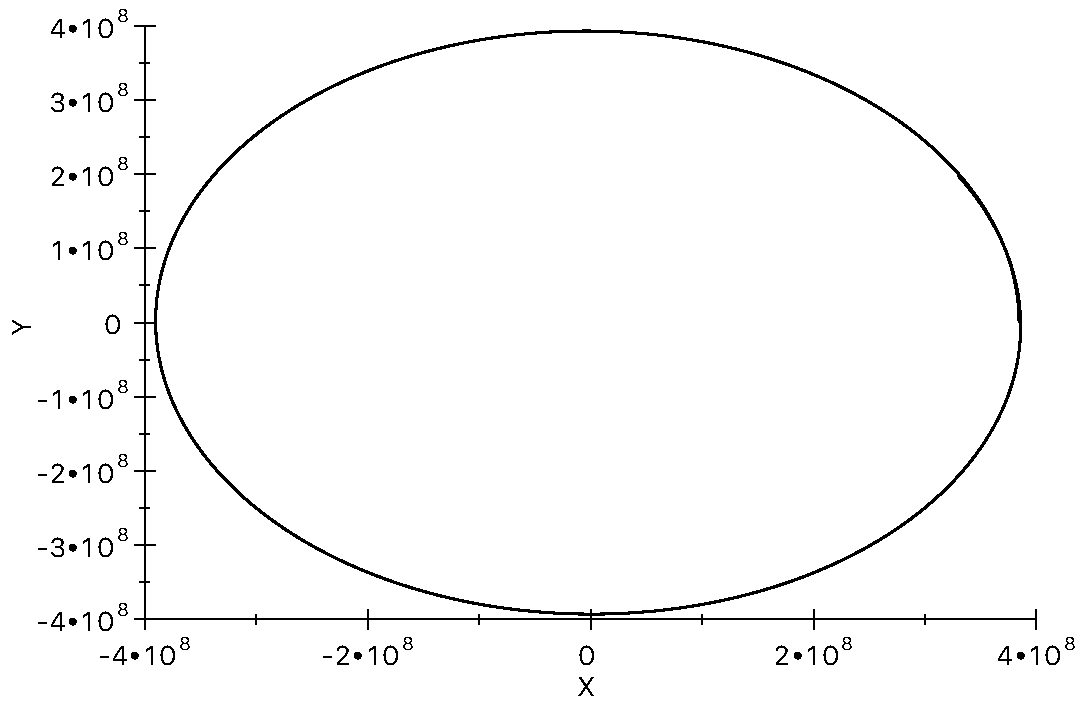
\includegraphics[width=1.\textwidth]{smalllooper.pdf}
		\caption{Motion of Moon around Earth} 
	\end{figure} 
In the end, we can see from the plots above the motion of the Earth and Moon system do indeed move about the Sun. Small deviations can be seen when moving in on this orbit, this are determined to be trajectories of the moon's orbit of the Earth happening at the same time. To highlight this motion it was asked that we plot the moon-earth orbit on a month scale seen in \textbf{Figure 3} (with small overlap in the far right). Few minor errors existed in compiling the final code such injection of the moon and misplacement of write statements, however these were fixed quickly and results then plotted. Finally with the resultant motion of the Sun Earth Moon system being computed, the use of the RK45 method and its adaptive step size allowed for correct and minimal deviations in the pathway and can be seen as a success.     
\newpage
\begin{thebibliography}{}
 \bibitem{1}
	Z.~Papp and A.~Bill, {\it Computational Physics Lecture Notes}, California State University Long Beach.

\end{thebibliography}
\end{document}








